%---------------------------
\begin{figure}[!tb]
\centering
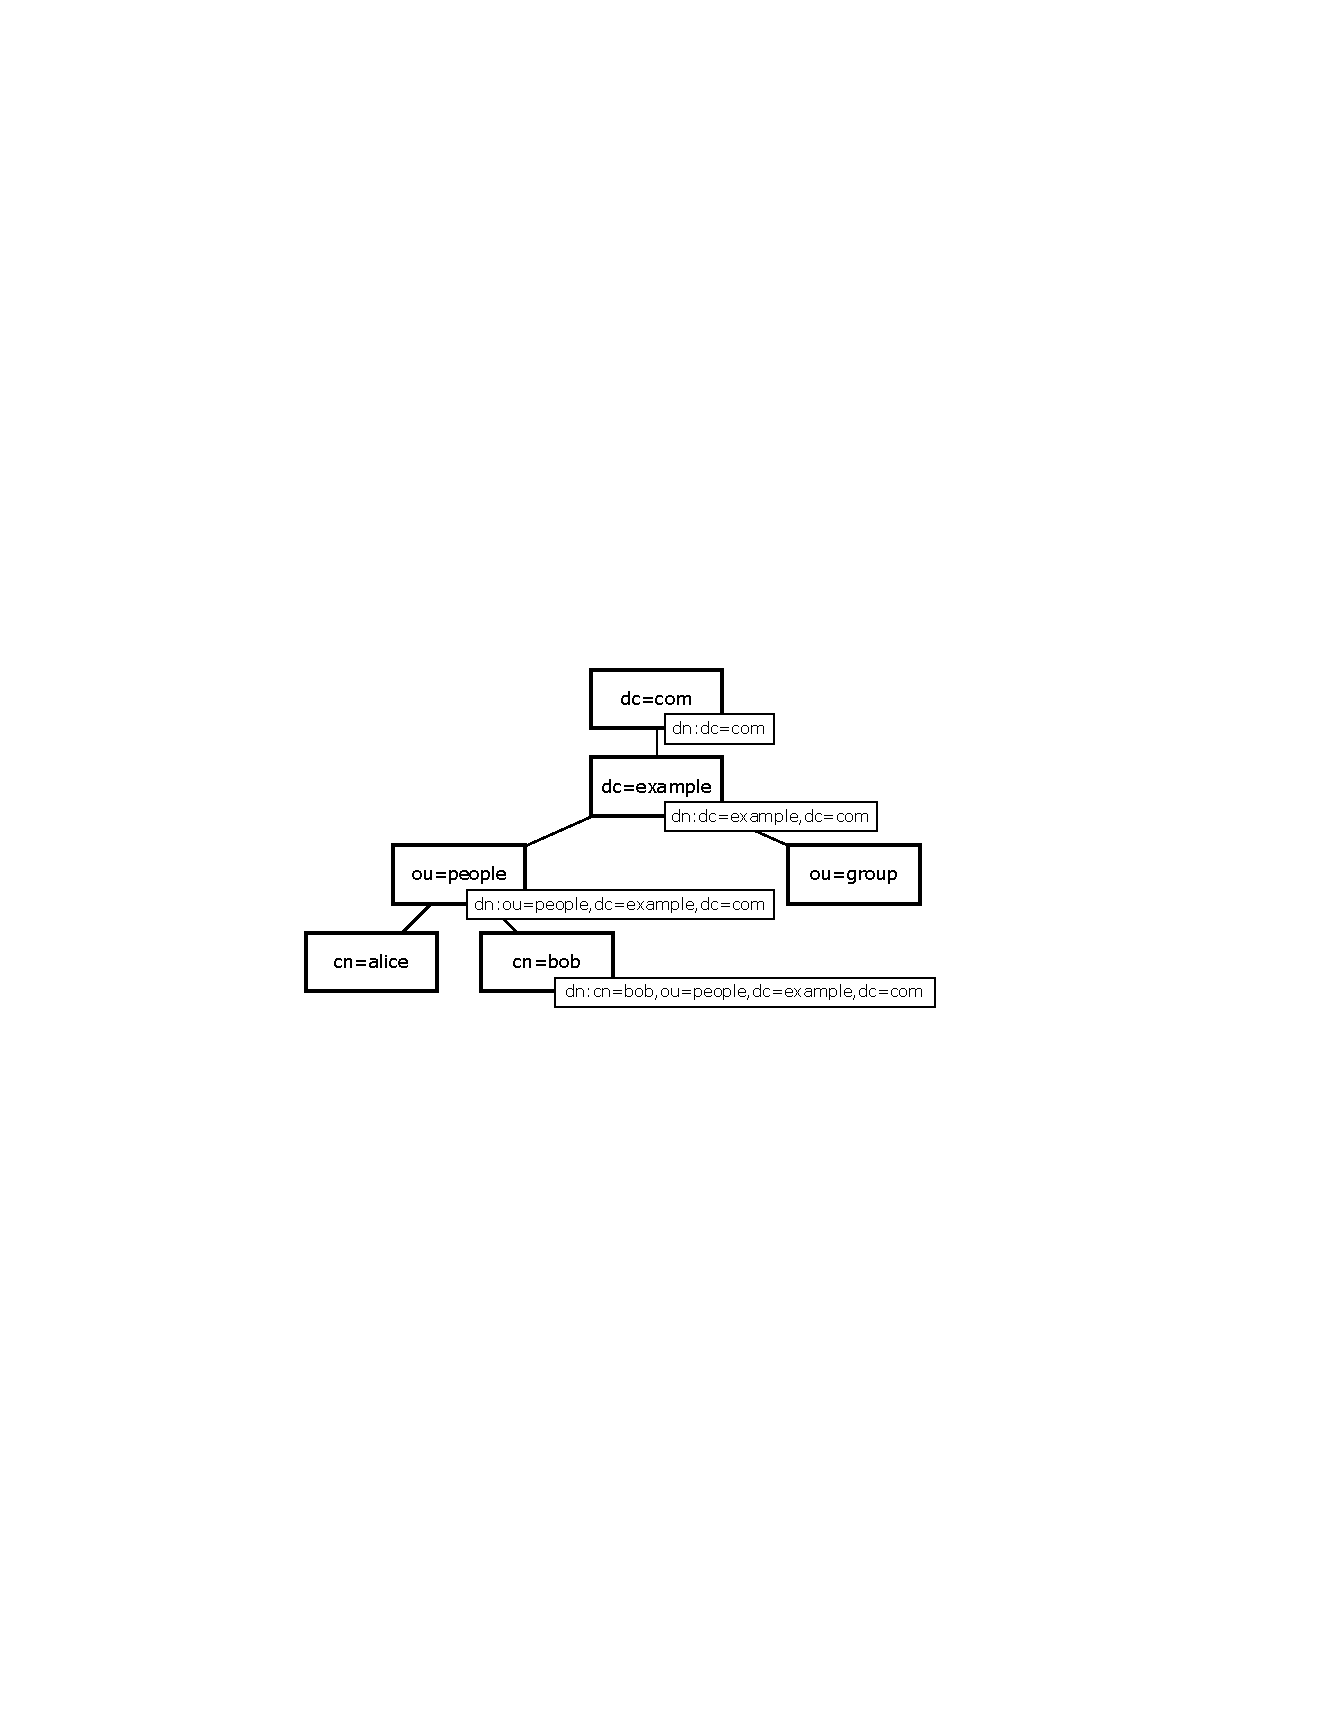
\includegraphics[width=\linewidth]{img/ldap_dit.pdf}
\caption{LDAP DIT example.}
\label{fig:DITExample}
\end{figure}
%% %---------------------------
%-------------------------------------------------------------------------------
\section{Background}
\label{sec:background}
%-------------------------------------------------------------------------------

\subsection{The Lightweight Directory Access Protocol (LDAP)}

%\subsubsection{Directory Architecture} The Lightweight Directory Access Protocol (LDAP) \cite{LDAP_RFC} serves as an access protocol designed for querying in X.500 and ISO/IEC 9594-1:2020 standardized directory services. These services store their data in a database called the Directory Information Base (DIB) \cite{x500standard} \cite{x501Standard} \cite{LDAP_RFC_Model}. The DIB organizes entries in the Directory Information Tree (DIT), as shown in \cref{fig:DITExample}. 
Data access using the \glsfirst{LDAP} assumes an X.500 directory structure, which uses a hierarchical tree structure called \gls{DIT}, as shown in \cref{fig:DITExample}.
Every entry within this directory system is identified by a distinct \gls{DN}. This \gls{DN} consists of the entry's name and the path leading back to the root entry---also known as the directory path. Additionally, entries have attributes with a predefined type and a value. The type determines the syntax, semantics, and characteristics of the value. Attribute types are uniquely identified internationally by their \gls{OID}~\cite{x500standard,x501Standard}.

The \gls{DSA}'s \gls{DSE} is the root node within the \gls{DIT}~\cite{LDAP_RFC_Model}. Clients can access this entry through a search operation specifying the desired attributes of the \gls{DSE}. These attributes hold a unique significance, as they encompass essential information about the server, such as supported controls, extensions, features, LDAP versions, SASL mechanisms, and more~\cite{LDAP_RFC_Model}.


%\subsubsection{Communications}
%\todo{Consider moving this info to the next paper, where we dive deeper into the LDAP protocol.}
%The exchange via the LDAP protocol involves two messages: the LDAPMessage from the client and the LDAPResult as the server's response. The LDAP Message includes an ID, an operation, and optionally, additional controls can be added. The following operations are supported: Bind, Unbind, Add, Search, Compare, Modify, Delete, Abandon, Extended Operation \cite{LDAP_RFC}.

%Controls are optional and are used to enhance an operation uniquely identified by an OID. If the server does not support the specified controls, the operation is aborted as long as the client has not marked the respective control as non-critical \cite{LDAP_RFC}.

% The LDAPResult comprises several components, including the resultCode, which offers a range of success and failure codes. In addition, the diagnostic message is an optional string that may hold further information regarding an operation, usually aiding in troubleshooting and error analysis. 
% \todo{Transition?} It also includes the matchedDN field, an optional DN representing the closest ancestor to the provided DN. For instance, if a request targets name=missing,dc=example,dc=com, the matchedDN would be dc=example,dc=com. Furthermore, there's the referral field, which is an optional list of one or more URIs that the client may employ for reattempting the operation. 
%These URIs may point to another server or a different location in the DIT \cite{LDAP_RFC}.

\subsection{LDAP Authentication and Authorization}

%LDAP itself does not inherently offer safeguards for accessing or modifying the directory server~\cite{RFC4512LDAPAuthenticationMethodsAndSecurityMechanisms}. However, servers may store sensitive data.  LDAP's cleartext password authentication method is strongly discouraged, especially when the transport service is not secure. SASL mechanisms do not offer adequate protection, either~~\cite{RFC4422SASL,
%RFC4512LDAPAuthenticationMethodsAndSecurityMechanisms, findlayBestPracticesLDAP, LDAP_RFC}.

Clients authenticate to an LDAP server by attempting a bind operation. A connection between the client and the server is established if the bind is successful~\cite{rfc4511, LDAP_RFC_AUTHENTICATION}. As part of the bind request, the client chooses an authentication method and, if necessary, supplies authentication credentials. LDAPv3 supports four types of authentication: simple, anonymous, unauthenticated, and SASL authentication~\cite{LDAP_RFC_AUTHENTICATION}. 

\textit{Simple Authentication} is performed when the client transmits the fully qualified DN of a user and a cleartext password. This method necessitates an encrypted channel, such as TLS, as transmitting the password in plaintext exposes it to the network~\cite{LDAP_RFC_AUTHENTICATION}.

\textit{Anonymous Authentication} uses empty values for both the username and password or sends a request without a prior bind operation. The client is then authenticated as an anonymous user. This anonymous bind is a mandatory part of the protocol~\cite{LDAP_RFC_AUTHENTICATION}.

\textit{Unauthenticated Authentication} is a simple authentication with a username and an empty password. The client is then bound as an unauthenticated user. It's worth noting that RFC 4513~\cite{LDAP_RFC_AUTHENTICATION} recommends disabling this method by default for clients and servers. This is due to the unexpected nature of users being able to bind without supplying a password, which may cause security issues. 

\paragraph{SASL.} SASL supports a wide range of authentication methods, such as username/password, Kerberos, and digital certificates. Anonymous and plaintext SASL authentication is not commonly used in LDAP~\cite{rfc4513}. While some are notably robust, others have been identified as insecure~\cite{RFC4422SASL}. 

Authorization, or access control, is not documented within the LDAP Standards~\cite{rfc4511}. Consequently, \gls{LDAP} server vendors often autonomously develop their own access control mechanisms. OpenLDAP uses \glspl{ACL}~\cite{alvinashcraftAccessControlLists2023, newellIntroductionLinuxAccess2020} for this purpose~\cite{OpenLDAPSoftwareAdministrator}.
%ACLs empower operating systems, software, and protocols to regulate access to data and functionalities, determining the extent to which a user may access objects and execute functions or services 
%\todo{\glspl{ACL} can be used to restrict access to nodes and attributes in the \gls{DIT} on OpenLDAP} 

\paragraph{LDAP as an Authentication Provider.}
LDAP is frequently used as a central component of single sign-on systems. For this purpose, most implementations follow a specific workflow: Initially, a search operation is initiated for the provided username to retrieve the \gls{DN} of the user's \gls{LDAP} entry. For this, LDAP servers must either allow unauthenticated searches or the application must use an authorized service account. Without the initial search, user sign-in becomes cumbersome because the user needs their Distinguished Name (DN), such as \texttt{CN=John Doe, OU=Users, DC=example, DC=com}.  After the search, the system proceeds to bind using the DN and the provided password. 

\subsection{Data Retrieval from LDAP Servers}

%\begin{todoenv}
%\begin{itemize}
%    \item Seach Operation: Grundlegende LDAP Operation, allows complex search queries, read attributes from specific entry, from subordinate entries or whole subtree (rfc 4511). Search is done on base object given by dn
%    \item SizeLimit 
%    \begin{itemize}
%        \item Server [can be set in config, defaults are: openldap: 500 (https://www.openldap.org/doc/admin24/limits.html) and apple: 11000 (https://support.apple.com/en-us/101250)] 
%        \item Client [RFC 4511 Section 4.5.1.4.  SearchRequest.sizeLimit]
%    \end{itemize}    
% \end{itemize}
%\end{todoenv}


The search operation is a fundamental feature of LDAP, enabling the retrieval of entries from an LDAP server. The search is performed relative to a base object entry, which the client specifies using a DN. This can also be the root entry of the LDAP directory. Additionally, the scope of the search can be restricted. This allows limiting the search to the specified entry, to the immediate subordinate level of the specified entry, or to its entire subtree.

The search criteria are determined by specifying search filters, based on which the search is conducted. For example, the filter \texttt{sn=Doe} searches for an entry where the attribute \texttt{sn} (surname) contains the value Doe. Multiple filters can be combined using logical operators such as AND, OR, or NOT. Additionally, searching for any value in an attribute is permissible by specifying an asterisk (\eg \texttt{sn=*}). Furthermore, the LDAP protocol allows for the specification of attributes in the search request that should be exclusively returned in the event of a match. It is possible to determine whether only the attribute names or both the attribute names and values should be returned.

Another option that can be specified in the search request is the size limit. This allows the client to determine the maximum number of results to be returned by the server in the event of a match. In addition to client-side size limits, various LDAP servers allow for server-side size limits to be configured to restrict the number of entries returned in a search request. Different LDAP server manufacturers establish different default values for size limits. For example, the default size in OpenLDAP is set at 500 entries, while Apple's Open Directory Server sets it at 11,000 entries.